\appendix
\section{Appendix}

\subsection{Example graph and first Nice Tree Decomposition}

Here we provide a detailed simulation of the dynamic programming algorithm.
\begin{figure}[h!]
    \centering
    
    \begin{minipage}{0.45\textwidth}
        \centering
        \begin{tikzpicture}
        \tikzstyle{vertex}=[circle, draw, minimum size=1cm, font=\small]

            \node[vertex] (a) at (0, 0) {a};
            \node[vertex] (b) at (-2, 2) {b};
            \node[vertex] (c) at (0, 4) {c};
            \node[vertex] (d) at (2, 2) {d};

            \draw (a) -- (b);
            \draw (b) -- (c);
            \draw (c) -- (d);
            \draw (d) -- (a);

            \node[below=0.2cm of a] {\small $1$};
            \node[left=0.2cm of b] {\small $3$};
            \node[above=0.2cm of c] {\small $4$};
            \node[right=0.2cm of d] {\small $2$};
        \end{tikzpicture}
        \caption{Weighted Rhombus Graph $G$}
        \label{fig:rhombus}
    \end{minipage}%
    \hfill
    \begin{minipage}{0.45\textwidth}
        \centering
        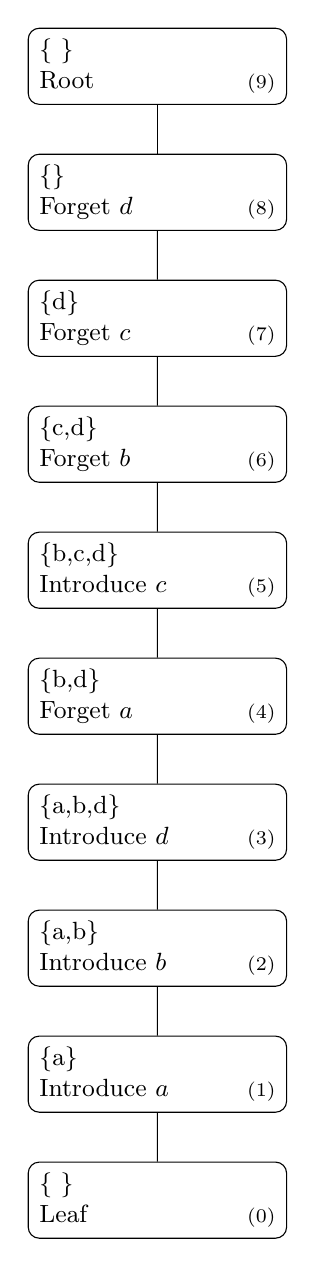
\begin{tikzpicture}[every node/.style={draw, rounded corners, align=left, font=\small, text width=3cm, inner sep=4pt}, level distance=1.6cm, sibling distance=5cm]
  
            \node (root) {\{ \} \\ Root \hfill \scriptsize(9)}
                child { node (f_d) {\{\} \\ Forget $d$ \hfill \scriptsize(8)}
                    child { node (f_c) {\{d\} \\ Forget $c$ \hfill \scriptsize(7)}
                        child { node (f_b) {\{c,d\} \\ Forget $b$ \hfill \scriptsize(6)}
                            child { node (i_c) {\{b,c,d\} \\ Introduce $c$ \hfill \scriptsize(5)}
                                child { node (f_a) {\{b,d\} \\ Forget $a$ \hfill \scriptsize(4)}
                                    child { node (i_d) {\{a,b,d\} \\ Introduce $d$ \hfill \scriptsize(3)}
                                        child { node (i_b) {\{a,b\} \\ Introduce $b$ \hfill \scriptsize(2)}
                                            child { node (i_a) {\{a\} \\ Introduce $a$ \hfill \scriptsize(1)}
                                                child { node (leaf) {\{ \} \\ Leaf \hfill \scriptsize(0)} }
                                            }
                                        }
                                    }
                                }
                            }
                        }
                    }
                };

        \end{tikzpicture}
        \caption{Nice Tree Decomposition of the Rhombus Graph}
        \label{fig:tree_decomposition}
    \end{minipage}
\end{figure}

\subsection{Simulation of Table Population}

The table \( c[\text{i}, I, \mathcal{F}] \) represents the population of the values as we move through the tree decomposition steps. Below, we provide a simulation of this process.

% First part of the table
\begin{minipage}{0.45\textwidth}
    \begin{longtable}{|c|c|c|c|}
    \hline
    \textbf{Index \(i\)} & \textbf{Set \(I\)} & \textbf{Flag \( \mathcal{F} \)} & \textbf{Value \( c[i, I, \mathcal{F}] \)} \\
    \hline
    \endfirsthead
    \hline
    \textbf{Index \(i\)} & \textbf{Set \(I\)} & \textbf{Flag \( \mathcal{F} \)} & \textbf{Value \( c[i, I, \mathcal{F}] \)} \\
    \hline
    \endhead
    \hline
    \endfoot
    % Leaf node
    0 & \( \emptyset \) & \( \emptyset \) & 0 \\
    \hline
    % Introduce a
    1 & \( a \) & \( \emptyset \) & 1 \\
    1 & \( \emptyset \) & \( \emptyset \) & 0 \\
    \hline
    % Introduce b
    2 & \( \{ a, b \} \) & \( \emptyset \) & 4 \\
    2 & \( \{ a \} \) & \( \emptyset \) & 1 \\
    2 & \( \{ b \} \) & \( \emptyset \) & 3 \\
    2 & \( \emptyset \) & \( \emptyset \) & 0 \\
    \hline
    % Introduce d
    3 & \( \{ a, b, d \} \) & \( \emptyset \) & 6 \\
    3 & \( \{ a, b \} \) & \( \emptyset \) & 4 \\
    3 & \( \{ a, d \} \) & \( \emptyset \) & 3 \\
    3 & \( \{ b, d \} \) & \( \emptyset \) & 5 \\
    3 & \( \{ a \} \) & \( \emptyset \) & 1 \\
    3 & \( \{ b \} \) & \( \emptyset \) & 3 \\
    3 & \( \{ d \} \) & \( \emptyset \) & 2 \\
    3 & \( \emptyset \) & \( \emptyset \) & 0 \\
    \hline
    % Forget a
    4 & \( \{ b, d \} \) & \( \emptyset \) & 6 \\
    4 & \( \{ b, d \} \) & \( \{ b, d \} \) & 5 \\
    
    4 & \( \{ b \} \) & \( \emptyset \) & 4 \\
    4 & \( \{ b \} \) & \( \{ b, d \} \) & 3 \\
    4 & \( \{ d \} \) & \( \emptyset \) & 3 \\
    4 & \( \{ d \} \) & \( \{ b, d \} \) & 2 \\
    4 & \( \emptyset \) & \( \emptyset \) & 1 \\
    4 & \( \emptyset \) & \( \{ b, d \} \) & 0 \\
    \hline

    % Introduce c
    5 & \( \{ b, c, d \} \) & \( \emptyset \) & 10 \\
    5 & \( \{ b, c, d \} \) & \( \{ b,d \} \) & 9 \\
    5 & \( \{ b, d \} \) & \( \emptyset \) & 6 \\
    5 & \( \{ b, d \} \) & \( \{ b, d \} \) & 5 \\
    \hline
    \end{longtable}
    \end{minipage}%
    \hfill
    % Second part of the table
    \begin{minipage}{0.45\textwidth}
    \begin{longtable}{|c|c|c|c|}
    \hline
    \textbf{Index \(i\)} & \textbf{Set \(I\)} & \textbf{Flag \( \mathcal{F} \)} & \textbf{Value \( c[i, I, \mathcal{F}] \)} \\
    \hline
    \endfirsthead
    \hline
    \textbf{Index \(i\)} & \textbf{Set \(I\)} & \textbf{Flag \( \mathcal{F} \)} & \textbf{Value \( c[i, I, \mathcal{F}] \)} \\
    \hline
    \endhead
    \hline
    \endfoot
    
    5 & \( \{ b, c \} \) & \( \emptyset \) & 8 \\
    5 & \( \{ b, c \} \) & \( \{ b, d \} \) & 7 \\
    5 & \( \{ b \} \) & \( \emptyset \) & 4 \\
    5 & \( \{ b \} \) & \( \{ b, d \} \) & 3 \\
    
    5 & \( \{ c, d \} \) & \( \emptyset \) & 7 \\
    5 & \( \{ c, d \} \) & \( \{ b, d \} \) & 6 \\
    5 & \( \{ d \} \) & \( \emptyset \) & 3 \\
    5 & \( \{ d \} \) & \( \{ b, d \} \) & 2 \\
    
    5 & \( \{ c \} \) & \( \emptyset \) & 5 \\
    5 & \( \{ c \} \) & \( \{ b, d \} \) & 4 \\
    5 & \( \emptyset \) & \( \emptyset \) & 1 \\
    5 & \( \emptyset \) & \( \{ b, d \} \) & \( \infty \) \\

    \hline
    % Forget b
    6 & \( \{ c, d \} \) & \( \emptyset \) & 10 \\
    6 & \( \{ c, d \} \) & \( \emptyset \) & 9 \\
    6 & \( \{ d \} \) & \( \emptyset \) & 6 \\
    6 & \( \{ d \} \) & \( \emptyset \) & 5 \\

    6 & \( \{ c \} \) & \( \emptyset \) & 8 \\
    6 & \( \{ c \} \) & \( \emptyset \) & 7 \\
    6 & \( \emptyset \) & \( \emptyset \) & 4 \\
    6 & \( \emptyset \) & \( \emptyset \) & 3 \\
    
    6 & \( \{ c, d \} \) & \( \emptyset \) & 7 \\
    6 & \( \{ c, d \} \) & \( \emptyset \) & 6 \\
    6 & \( \{ d \} \) & \( \emptyset \) & 3 \\
    6 & \( \{ d \} \) & \( \emptyset \) & 2 \\

    6 & \( \{ c \} \) & \( \emptyset \) & 5 \\
    6 & \( \{ c \} \) & \( \emptyset \) & 4 \\
    6 & \( \emptyset \) & \( \emptyset \) & 1 \\
    6 & \( \emptyset \) & \( \emptyset \) & \( \infty \) \\

    \hline
    \end{longtable}
\end{minipage}

Notice that at this point, at index 6, we are taking minimum values that we can resolve. 
That is, some values can be thrown out, because they are suboptimal.

\begin{minipage}{0.48\textwidth}
    \begin{longtable}{|c|c|c|c|}
    \hline
    \textbf{Index \(i\)} & \textbf{Set \(I\)} & \textbf{Flag \( \mathcal{F} \)} & \textbf{Value \( c[i, I, \mathcal{F}] \)} \\
    \hline
    \endfirsthead
    \hline
    \textbf{Index \(i\)} & \textbf{Set \(I\)} & \textbf{Flag \( \mathcal{F} \)} & \textbf{Value \( c[i, I, \mathcal{F}] \)} \\
    \hline
    \endhead
    \hline
    \endfoot

    % Forget b
    6 & \( \{ c, d \} \) & \( \emptyset \) & 6 \\
    6 & \( \{ d \} \) & \( \emptyset \) & 2 \\
    6 & \( \{ c \} \) & \( \emptyset \) & 4 \\
    6 & \( \emptyset \) & \( \emptyset \) & 1 \\
    \hline
    \end{longtable}
\end{minipage}
\hfill
\begin{minipage}{0.48\textwidth}
    \begin{longtable}{|c|c|c|c|}
    \hline
    \textbf{Index \(i\)} & \textbf{Set \(I\)} & \textbf{Flag \( \mathcal{F} \)} & \textbf{Value \( c[i, I, \mathcal{F}] \)} \\
    \hline
    \endfirsthead
    \hline
    \textbf{Index \(i\)} & \textbf{Set \(I\)} & \textbf{Flag \( \mathcal{F} \)} & \textbf{Value \( c[i, I, \mathcal{F}] \)} \\
    \hline
    \endhead
    \hline
    \endfoot

    % Forget c
    7 & \( \{ d \} \) & \( \emptyset \) & 2 \\
    7 & \( \emptyset \) & \( \emptyset \) & 1 \\
    \hline
    % Forget d
    8 & \( \emptyset \) & \( \emptyset \) & 1 \\
    \hline
    % Final
    9 & \( \emptyset \) & \( \emptyset \) & 1 \\
    \hline
    \end{longtable}
\end{minipage}

There is one value at the root and it is the minimum weight of a set $F$ that breaks 
every 4-cycle in a planar graph $G$.

\newpage

\subsection{Example graph and second Nice Tree Decomposition}

Here we offer a different nice tree decomposition, so we can inspect what happens at a join 
node.

\begin{figure}[h]
    \centering
    \begin{minipage}{0.45\textwidth}
        \centering
        \begin{tikzpicture}
        \tikzstyle{vertex}=[circle, draw, minimum size=1cm, font=\small]

            \node[vertex] (a) at (0, 0) {a};
            \node[vertex] (b) at (-2, 2) {b};
            \node[vertex] (c) at (0, 4) {c};
            \node[vertex] (d) at (2, 2) {d};

            \draw (a) -- (b);
            \draw (b) -- (c);
            \draw (c) -- (d);
            \draw (d) -- (a);

            \node[below=0.2cm of a] {\small $1$};
            \node[left=0.2cm of b] {\small $3$};
            \node[above=0.2cm of c] {\small $4$};
            \node[right=0.2cm of d] {\small $2$};
        \end{tikzpicture}
        \caption{Weighted Rhombus Graph $G$}
        \label{fig:rhombus2}
    \end{minipage}%
    \hfill
    \begin{minipage}{0.45\textwidth}
        \centering
        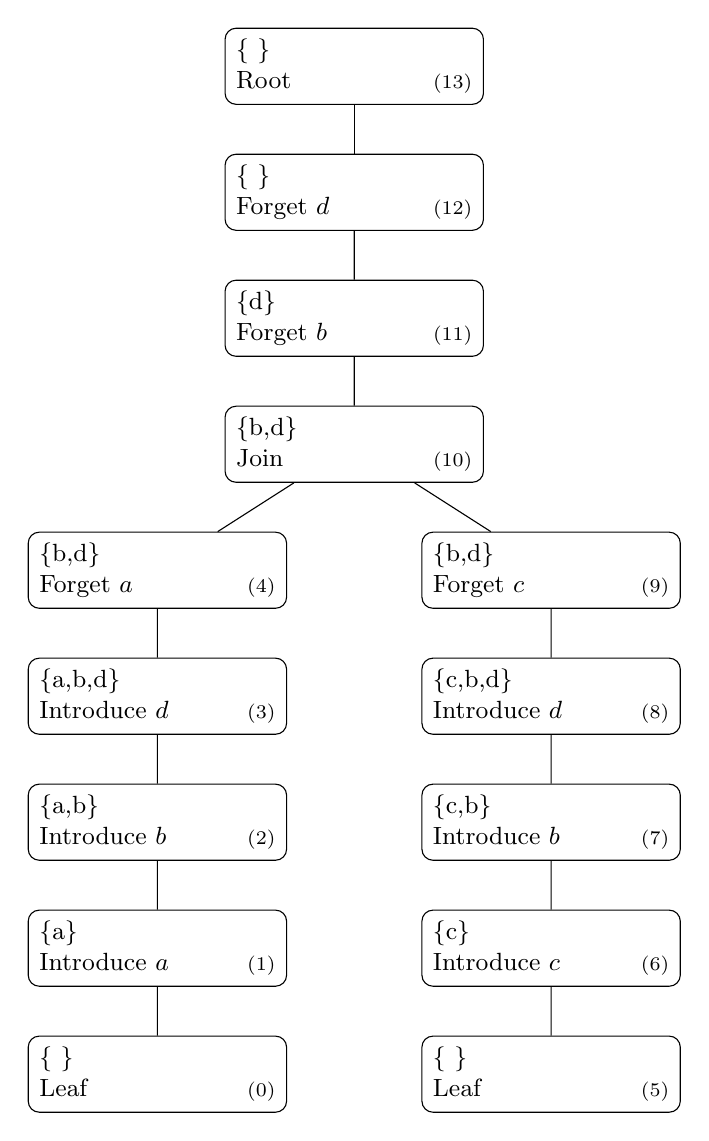
\begin{tikzpicture}[every node/.style={draw, rounded corners, align=left, font=\small, text width=3cm, inner sep=4pt}, level distance=1.6cm, sibling distance=5cm]

            \node (root) {\{ \} \\ Root \hfill \scriptsize(13) }
                child { node (f_d) {\{ \} \\ Forget $d$ \hfill \scriptsize(12)}
                    child { node (f_b) {\{d\} \\ Forget $b$ \hfill \scriptsize(11)}
                        child { node (join) {\{b,d\} \\ Join \hfill \scriptsize(10)}
                            child { node (path1) {\{b,d\} \\ Forget $a$ \hfill \scriptsize(4)}
                                child { node (i_b1) {\{a,b,d\} \\ Introduce $d$ \hfill \scriptsize(3)}
                                    child { node (i_d1) {\{a,b\} \\ Introduce $b$ \hfill \scriptsize(2)}
                                        child { node (i_a) {\{a\} \\ Introduce $a$ \hfill \scriptsize(1)}
                                            child { node (leaf1) {\{ \} \\ Leaf \hfill \scriptsize(0)} }
                                        }
                                    }
                                }
                            }
                        child { node (path2) {\{b,d\} \\ Forget $c$ \hfill \scriptsize(9)}
                            child { node (i_b2) {\{c,b,d\} \\ Introduce $d$ \hfill \scriptsize(8)}
                                child { node (i_d2) {\{c,b\} \\ Introduce $b$ \hfill \scriptsize(7)}
                                    child { node (i_c) {\{c\} \\ Introduce $c$ \hfill \scriptsize(6)}
                                        child { node (leaf2) {\{ \} \\ Leaf \hfill \scriptsize(5)} }
                                    }
                                }
                            }
                        }
                    }
                }
            };

        \end{tikzpicture}
        \caption{Alternative Tree Decomposition with Join Node at \{b,d\}}
        \label{fig:alt_tree_decomposition}
    \end{minipage}
\end{figure}

\subsection{Simulation of Table Population of graph two}

Up until the join node, the calculation of the dynamic programming table is standard.

\begin{minipage}[t]{0.48\textwidth} % [t] for top alignment
    \centering
    \begin{longtable}{|c|c|c|c|}
        \hline
        \textbf{Index $i$} & \textbf{Set $I$} & \textbf{Flag $\mathcal{F}$} & \textbf{Value $c[i, I, \mathcal{F}]$} \\
        \hline
        \endfirsthead
        \hline
        \textbf{Index $i$} & \textbf{Set $I$} & \textbf{Flag $\mathcal{F}$} & \textbf{Value $c[i, I, \mathcal{F}]$} \\
        \hline
        \endhead
        \hline
        \endfoot

        \hline
        0 & $\emptyset$ & $\emptyset$ & \textbf{0} \\
        \hline
        1 & $\{a\}$ & $\emptyset$ & \textbf{1} \\
        1 & $\emptyset$ & $\emptyset$ & \textbf{0} \\
        \hline
        2 & $\{a,b\}$ & $\emptyset$ & \textbf{4} \\
        2 & $\{a\}$ & $\emptyset$ & \textbf{1} \\
        2 & $\{b\}$ & $\emptyset$ & \textbf{3} \\
        2 & $\emptyset$ & $\emptyset$ & \textbf{0} \\
        \hline
        3 & $\{a,b,d\}$ & $\emptyset$ & \textbf{6} \\
        3 & $\{a,b\}$ & $\emptyset$ & \textbf{4} \\
        3 & $\{a,d\}$ & $\emptyset$ & \textbf{3} \\
        3 & $\{b,d\}$ & $\emptyset$ & \textbf{5} \\
        3 & $\{a\}$ & $\emptyset$ & \textbf{1} \\
        3 & $\{b\}$ & $\emptyset$ & \textbf{3} \\
        3 & $\{d\}$ & $\emptyset$ & \textbf{2} \\
        3 & $\emptyset$ & $\emptyset$ & \textbf{0} \\
        \hline
        4 & $\{b,d\}$ & $\emptyset$ & \textbf{6} \\
        4 & $\{b,d\}$ & $\{b,d\}$ & \textbf{5} \\
        4 & $\{b\}$ & $\emptyset$ & \textbf{4} \\
        4 & $\{b\}$ & $\{b,d\}$ & \textbf{3} \\
        4 & $\{d\}$ & $\emptyset$ & \textbf{3} \\
        4 & $\{d\}$ & $\{b,d\}$ & \textbf{2} \\
        4 & $\emptyset$ & $\emptyset$ & \textbf{1} \\
        4 & $\emptyset$ & $\{b,d\}$ & \textbf{0} \\
        \hline
    \end{longtable}
\end{minipage}%
\hfill
\begin{minipage}[t]{0.48\textwidth} % [t] for top alignment
    \centering
    \begin{longtable}{|c|c|c|c|}
        \hline
        \textbf{Index $i$} & \textbf{Set $I$} & \textbf{Flag $\mathcal{F}$} & \textbf{Value $c[i, I, \mathcal{F}]$} \\
        \hline
        \endfirsthead
        \hline
        \textbf{Index $i$} & \textbf{Set $I$} & \textbf{Flag $\mathcal{F}$} & \textbf{Value $c[i, I, \mathcal{F}]$} \\
        \hline
        \endhead
        \hline
        \endfoot

        5 & $\emptyset$ & $\emptyset$ & \textbf{0} \\
        \hline
        6 & $\{c\}$ & $\emptyset$ & \textbf{4} \\
        6 & $\emptyset$ & $\emptyset$ & \textbf{0} \\
        \hline
        7 & $\{c,b\}$ & $\emptyset$ & \textbf{7} \\
        7 & $\{c\}$ & $\emptyset$ & \textbf{4} \\
        7 & $\{b\}$ & $\emptyset$ & \textbf{3} \\
        7 & $\emptyset$ & $\emptyset$ & \textbf{0} \\
        \hline
        8 & $\{c,b,d\}$ & $\emptyset$ & \textbf{9} \\
        8 & $\{c,b\}$ & $\emptyset$ & \textbf{7} \\
        8 & $\{c,d\}$ & $\emptyset$ & \textbf{6} \\
        8 & $\{b,d\}$ & $\emptyset$ & \textbf{5} \\
        8 & $\{c\}$ & $\emptyset$ & \textbf{4} \\
        8 & $\{b\}$ & $\emptyset$ & \textbf{3} \\
        8 & $\{d\}$ & $\emptyset$ & \textbf{2} \\
        8 & $\emptyset$ & $\emptyset$ & \textbf{0} \\
        \hline
        9 & $\{b,d\}$ & $\emptyset$ & \textbf{9} \\
        9 & $\{b,d\}$ & $\{b,d\}$ & \textbf{5} \\
        9 & $\{b\}$ & $\emptyset$ & \textbf{7} \\
        9 & $\{b\}$ & $\{b,d\}$ & \textbf{3} \\
        9 & $\{d\}$ & $\emptyset$ & \textbf{6} \\
        9 & $\{d\}$ & $\{b,d\}$ & \textbf{2} \\
        9 & $\emptyset$ & $\emptyset$ & \textbf{4} \\
        9 & $\emptyset$ & $\{b,d\}$ & \textbf{0} \\
        \hline
    \end{longtable}
\end{minipage}

Now we have to calculate the join node. Note that we will not write out every value and only 
then take the minimum, but write the minimum values in the table directly.

\begin{minipage}[t]{0.48\textwidth} % [t] for top alignment
    \centering
    \begin{longtable}{|c|c|c|c|}
        \hline
        \textbf{Index $i$} & \textbf{Set $I$} & \textbf{Flag $\mathcal{F}$} & \textbf{Value $c[i, I, \mathcal{F}]$} \\
        \hline
        \endfirsthead
        \hline
        \textbf{Index $i$} & \textbf{Set $I$} & \textbf{Flag $\mathcal{F}$} & \textbf{Value $c[i, I, \mathcal{F}]$} \\
        \hline
        \endhead
        \hline
        \endfoot

        \hline
        10 & $\{b,d\}$ & $\emptyset$ & \textbf{10} \\
        10 & $\{b,d\}$ & $\{b,d\}$ & \textbf{5} \\
        10 & $\{b\}$ & $\emptyset$ & \textbf{8} \\
        10 & $\{b\}$ & $\{b,d\}$ & \textbf{3} \\
        10 & $\{d\}$ & $\emptyset$ & \textbf{7} \\
        10 & $\{d\}$ & $\{b,d\}$ & \textbf{2} \\

        \hline
    \end{longtable}
\end{minipage}%
\hfill
\begin{minipage}[t]{0.48\textwidth} % [t] for top alignment
    \centering
    \begin{longtable}{|c|c|c|c|}
        \hline
        \textbf{Index $i$} & \textbf{Set $I$} & \textbf{Flag $\mathcal{F}$} & \textbf{Value $c[i, I, \mathcal{F}]$} \\
        \hline
        \endfirsthead
        \hline
        \textbf{Index $i$} & \textbf{Set $I$} & \textbf{Flag $\mathcal{F}$} & \textbf{Value $c[i, I, \mathcal{F}]$} \\
        \hline
        \endhead
        \hline
        \endfoot

        10 & $\emptyset$ & $\emptyset$ & \textbf{5} \\
        10 & $\emptyset$ & $\{b,d\}$ & \textbf{1} \\
        \hline
        11 & $\{d\}$ & $\emptyset$ & \textbf{2} \\
        11 & $\emptyset$ & $\emptyset$ & \textbf{1} \\
        \hline
        12 & $\emptyset$ & $\emptyset$ & \textbf{1} \\
        \hline
        13 & $\emptyset$ & $\emptyset$ & \textbf{1} \\
        \hline
        
    \end{longtable}
\end{minipage}

